\documentclass[a4paper,12pt]{article}

% Setting up the geometry for the document
\usepackage[margin=1in]{geometry}

% Including essential packages for mathematical typesetting and tables
\usepackage{amsmath, amssymb}
\usepackage{booktabs}
\usepackage{array}
\usepackage{graphicx} % For including images
\usepackage{caption} % For better caption control
\usepackage{subcaption} % For subfigures
\usepackage{siunitx} % For formatting numbers and units
\usepackage{enumitem} % For better enumeration
\usepackage{hyperref} % For hyperlinks
\usepackage{xcolor} % For colored text
\usepackage{fancyhdr} % For custom headers and footers
\usepackage{float} % For better control of float placement
\usepackage{url} % For proper URL formatting

% Setting up the font
\usepackage{mathpazo} % Palatino font with math support

% Ensuring proper spacing and formatting
\usepackage{parskip}
\setlength{\parindent}{0pt}
\setlength{\parskip}{1em}

% Setting up the footer with name
\pagestyle{fancy}
\fancyhf{} % Clear default headers/footers
\fancyfoot[R]{Mohammad Hafizur Rahman Sakib}
\renewcommand{\headrulewidth}{0pt} % No header rule
\renewcommand{\footrulewidth}{0.4pt} % Thin footer rule

% Adding packages for better compatibility
\usepackage[T1]{fontenc} % Better font encoding
\usepackage[utf8]{inputenc} % UTF-8 encoding for special characters
\usepackage{microtype} % Improved typography

% Listings package for pseudocode / code blocks
\usepackage{listings}
\lstset{
    basicstyle=\ttfamily\small,
    breaklines=true,        % Automatic line breaking
    breakatwhitespace=true,
    frame=single,           % Frame around code
    backgroundcolor=\color{gray!10},
    tabsize=4,
    columns=fullflexible,
    keepspaces=true,
    showstringspaces=false
}

\hypersetup{
    colorlinks=true,
    linkcolor=blue,
    filecolor=magenta,
    urlcolor=cyan,
}

\begin{document}

% Title and Introduction
\section*{Introduction}
This lab report, titled \textbf{Build Convolution Neural Network with TensorFlow and Keras}, evaluates neural network models on the Pima Indians Diabetes Dataset and the Cassava Plant Disease Dataset. For the diabetes dataset, a regularized model with dropout and batch normalization was implemented, trained with Adam and SGD optimizers, and utilized early stopping to mitigate overfitting. For the Cassava dataset, two convolutional neural network (CNN) models were developed: a custom CNN and a pre-trained ResNet50 model, both incorporating data augmentation and early stopping. This report details dataset preprocessing, model architectures, training processes, and performance analysis through accuracy and loss curves, as well as overfitting assessments, highlighting the impact of regularization and data augmentation.

% Section 1: Details of the Datasets
\section*{Details of the Datasets}

\subsection*{Pima Indians Diabetes Dataset}
The Pima Indians Diabetes Dataset, sourced from the UCI Machine Learning Repository, contains 768 instances with 8 feature attributes and 1 binary target variable (Outcome: 1 for diabetes, 0 for no diabetes). The features include:
\begin{itemize}
    \item Pregnancies: Number of times pregnant.
    \item Glucose: Plasma glucose concentration (mg/dL).
    \item BloodPressure: Diastolic blood pressure (mm Hg).
    \item SkinThickness: Triceps skin fold thickness (mm).
    \item Insulin: 2-hour serum insulin (mu U/ml).
    \item BMI: Body mass index (weight in kg/(height in m)$^2$).
    \item DiabetesPedigreeFunction: Genetic predisposition to diabetes.
    \item Age: Age of the patient (years).
\end{itemize}
Missing values (zeros in Glucose, BloodPressure, SkinThickness, Insulin, and BMI) were replaced with column means, and features were normalized using StandardScaler.

\clearpage % Ensure clean page break before next section

\section*{Neural Network Model for Diabetes Dataset}
A regularized model was implemented using TensorFlow/Keras in Google Colab, trained with Adam and SGD optimizers, and incorporated early stopping (patience=10, monitoring validation loss).

\subsection*{Regularized Model with Dropout and Normalization}
The regularized model uses dropout (20\% rate) and batch normalization to enhance generalization and training stability.

\textbf{Pseudocode:}
\begin{lstlisting}
# Preprocess data
Load dataset
Replace zeros with mean in [Glucose, BloodPressure, SkinThickness, Insulin, BMI]
Set features X (all except Outcome), target y (Outcome)
Split data: 80% train, 20% test
Normalize features with StandardScaler

# Define early stopping
Monitor validation loss, patience 10 epochs, restore best weights

# Define model
Sequential model:
    Layer 1: 8 neurons, ReLU, input 8 features
    BatchNormalization
    Dropout (0.2)
    Layer 2: 4 neurons, ReLU
    BatchNormalization
    Dropout (0.2)
    Output: 1 neuron, sigmoid

# Train with Adam
Compile: Adam optimizer, binary crossentropy, accuracy
Train: 100 epochs, batch 32, early stopping
Store history (Adam)

# Train with SGD
Compile: SGD optimizer, binary crossentropy, accuracy
Train: 100 epochs, batch 32, early stopping
Store history (SGD)
\end{lstlisting}

\subsection*{Regularized Model Performance}
\begin{figure}[H]
    \centering
    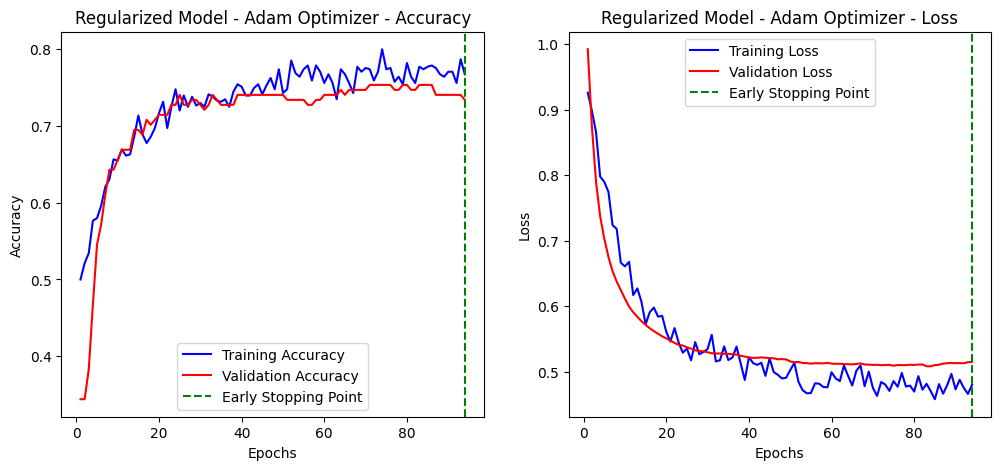
\includegraphics[width=1.0\textwidth]{assets/diabetes/adam_diabetes_loss.png}
    \caption{Accuracy of the Regularized Model (Adam and SGD Optimizers)}
\end{figure}

\begin{figure}[H]
    \centering
    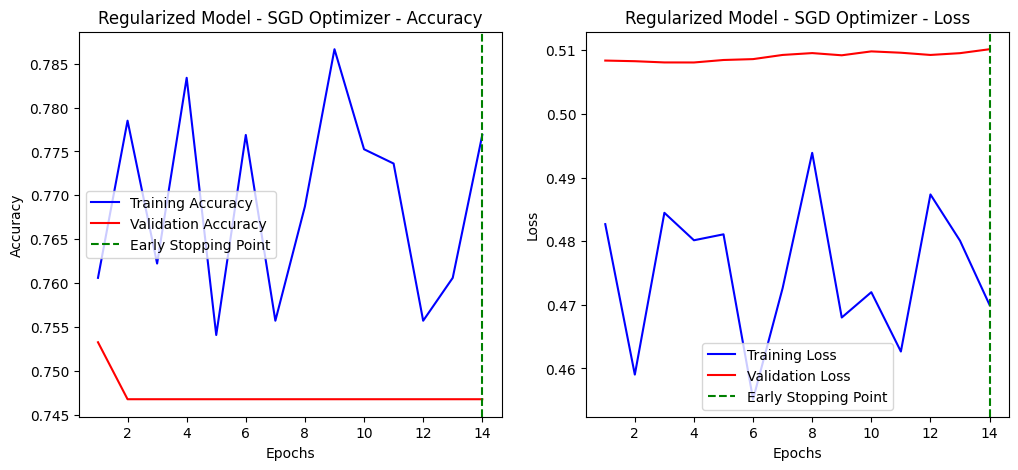
\includegraphics[width=1.0\textwidth]{assets/diabetes/sgd_diabetes_loss.png}
    \caption{Loss of the Regularized Model (Adam and SGD Optimizers)}
\end{figure}

\clearpage

\subsection*{Cassava Plant Disease Dataset Details}
The Cassava Plant Disease Dataset contains images of cassava leaves, labeled into five classes: Cassava Bacterial Blight (CBB), Cassava Brown Streak Disease (CBSD), Cassava Green Mottle (CGM), Cassava Mosaic Disease (CMD), and Healthy. The dataset includes:
\begin{itemize}
    \item \textbf{train\_images}: Folder with images resized to 224x224 pixels (RGB).
    \item \textbf{label\_num\_to\_disease\_map.json}: JSON file mapping labels (0–4) to disease names.
    \begin{itemize}
    \item[0:] Cassava Bacterial Blight (CBB)
    \item[1:] Cassava Brown Streak Disease (CBSD)
    \item[2:] Cassava Green Mottle (CGM)
    \item[3:] Cassava Mosaic Disease (CMD)
    \item[4:] Healthy
\end{itemize}

    \item \textbf{train.csv}: CSV file mapping image filenames to labels.For example : 
    \begin{table}[h!]
\centering
% Increase row height
\renewcommand{\arraystretch}{1.5}
% Increase column padding
\setlength{\tabcolsep}{44pt}

\begin{tabular}{|c|c|}
\hline
\textbf{image\_id} & \textbf{label} \\ \hline
1000015157.jpg & 0 \\ \hline
1000201771.jpg & 2 \\ \hline
100042118.jpg  & 1 \\ \hline
1000723321.jpg & 1 \\ \hline
1000812911.jpg & 4 \\ \hline
1000837476.jpg & 3 \\ \hline
\end{tabular}
\caption{Sample image IDs with corresponding labels}
\label{tab:sample_labels}
\end{table}

\end{itemize}
The dataset comprises approximately 21,000 images, with about 20\% per class, split into 80\% training and 20\% testing. Images were normalized to [0,1], and data augmentation was applied.

\subsubsection*{Sample Images}
\begin{figure}[H]
    \centering
    \begin{subfigure}{0.45\textwidth}
        \centering
        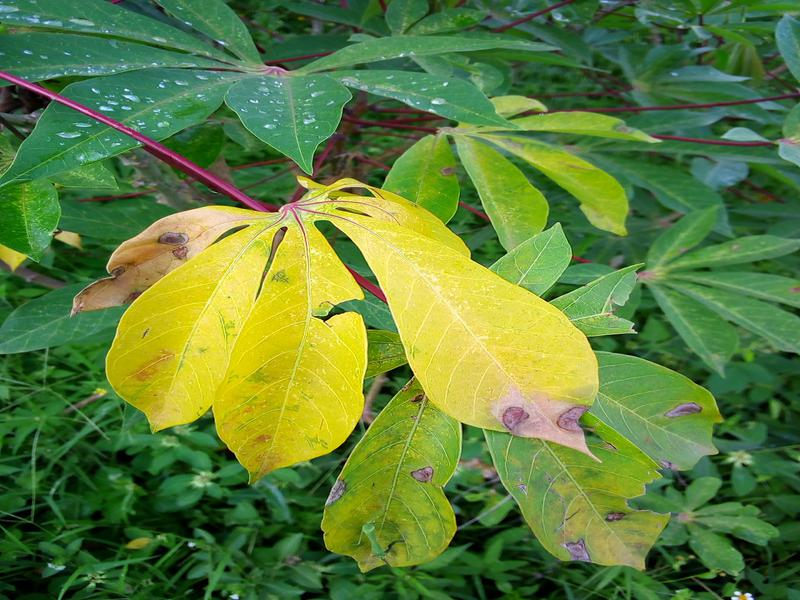
\includegraphics[width=\textwidth]{assets/class_images/class_0.jpg}
        \caption{Cassava Bacterial Blight (CBB)}
    \end{subfigure}\hfill
    \begin{subfigure}{0.45\textwidth}
        \centering
        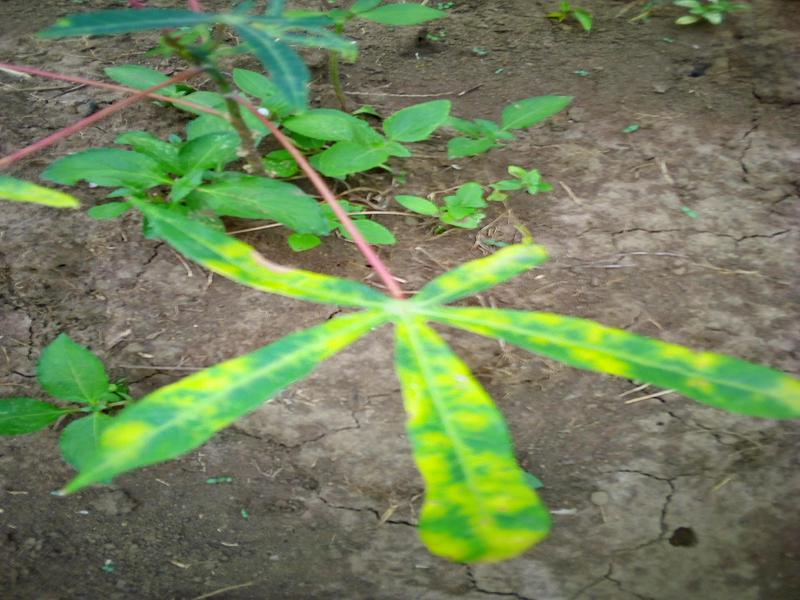
\includegraphics[width=\textwidth]{assets/class_images/class_1.jpg}
        \caption{Cassava Brown Streak Disease (CBSD)}
    \end{subfigure}
    
    \vspace{0.5cm}
    
    \begin{subfigure}{0.45\textwidth}
        \centering
        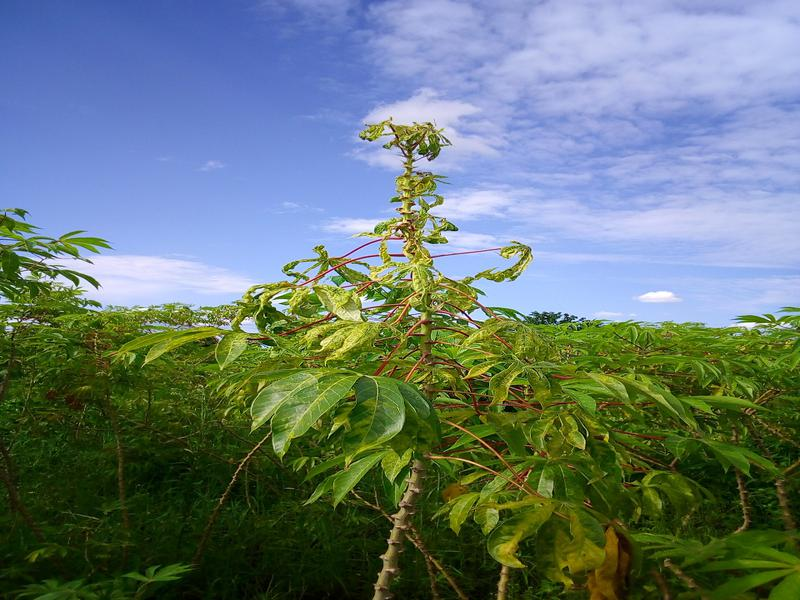
\includegraphics[width=\textwidth]{assets/class_images/class_2.jpg}
        \caption{Cassava Green Mottle (CGM)}
    \end{subfigure}\hfill
    \begin{subfigure}{0.45\textwidth}
        \centering
        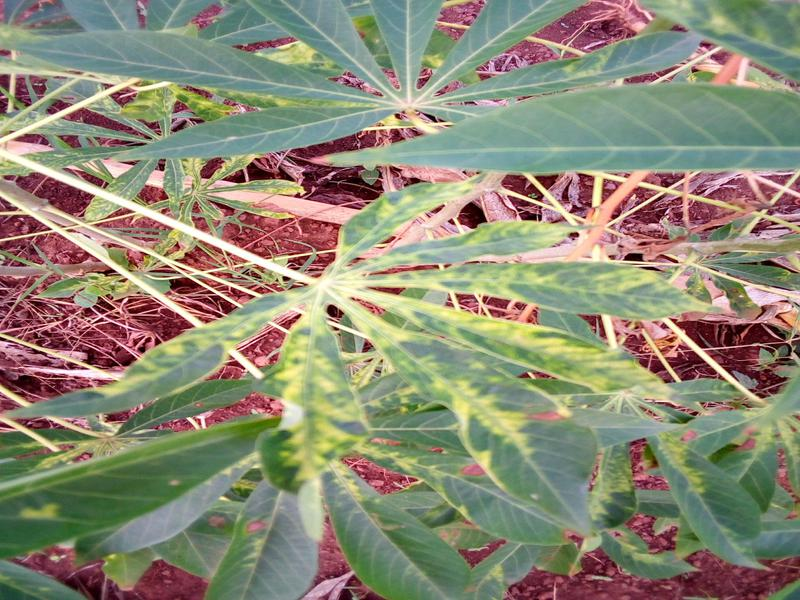
\includegraphics[width=\textwidth]{assets/class_images/class_3.jpg}
        \caption{Cassava Mosaic Disease (CMD)}
    \end{subfigure}
    
    \vspace{0.5cm}
    
    \begin{subfigure}{0.45\textwidth}
        \centering
        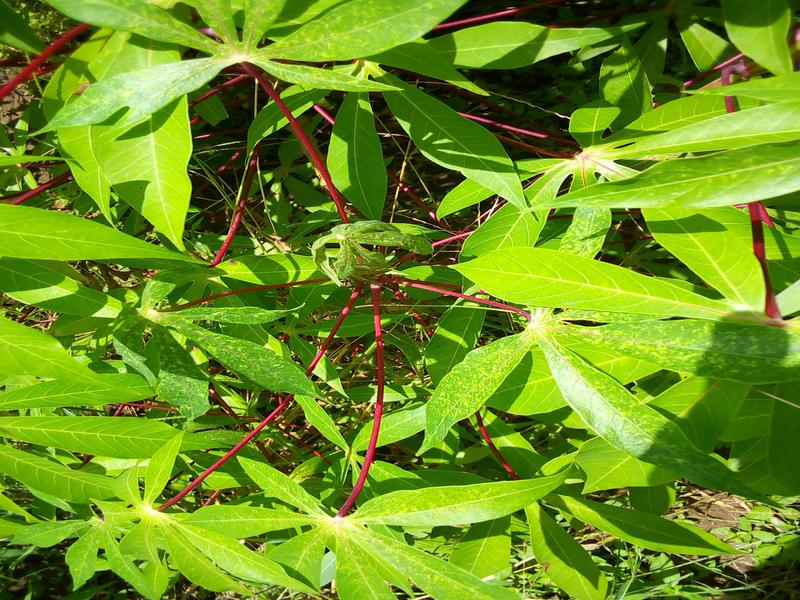
\includegraphics[width=\textwidth]{assets/class_images/class_4.jpg}
        \caption{Healthy}
    \end{subfigure}
    \caption{Sample images from the Cassava Plant Disease Dataset}
\end{figure}

\clearpage

\section*{Target and Feature Selection}
\subsection*{Cassava Plant Disease Dataset}
The target is a categorical label (0: CBB, 1: CBSD, 2: CGM, 3: CMD, 4: Healthy). Features are pixel intensities from 224x224x3 images, normalized with data augmentation applied.

\section*{Neural Network Models for Cassava Dataset}
Two CNN models were implemented: a custom CNN and a pre-trained ResNet50 model, both utilizing data augmentation and early stopping (patience=10, monitoring validation loss) to address overfitting and underfitting. Models were trained with the Adam optimizer in Google Colab.

\subsection*{Data Augmentation}
Data augmentation enhances model robustness with:
\begin{itemize}
    \item Rotation: Up to 20 degrees.
    \item Horizontal Flip: Randomly flip images.
    \item Zoom: Up to 20\% zoom range.
    \item Shear: Up to 20\% shear range.
\end{itemize}

\begin{figure}[H]
    \centering
    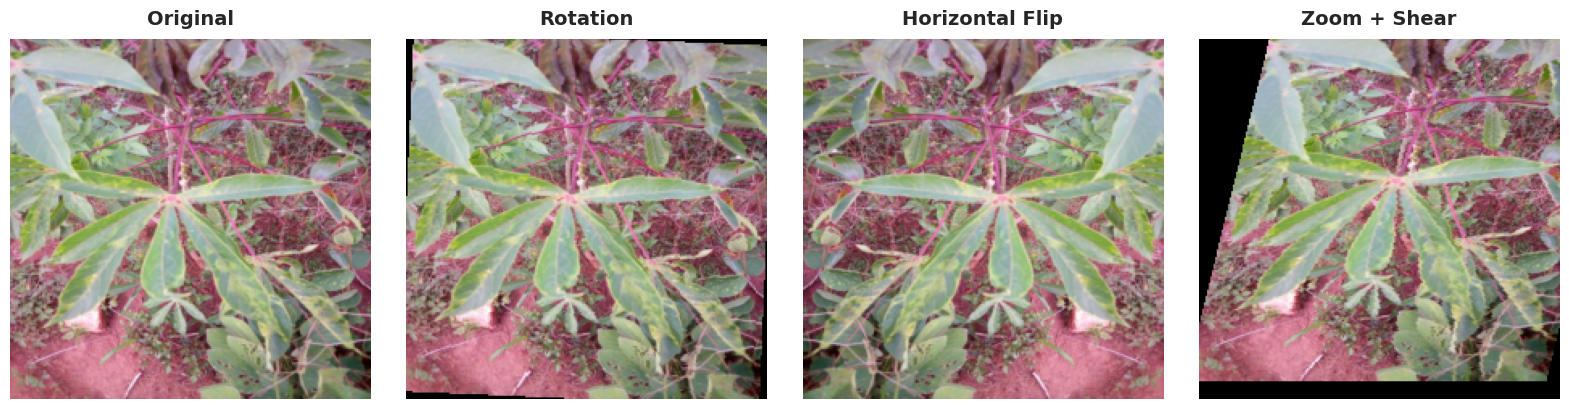
\includegraphics[width=0.8\textwidth]{assets/cassava/data_aug.png}
    \caption{Examples of Augmented Cassava Images (Rotation, Flip, Zoom, Shear)}
\end{figure}

\subsection*{Custom CNN Model}
\begin{lstlisting}
# Preprocess data
Load train.csv, train_images, label_map.json
Resize images to 224x224, normalize
Augment: rotate, flip, zoom
Split: 1000 train, 10 val, 200 test
Create DataLoaders: batch 32 (train), 10 (val), 32 (test)

# Early stopping
Monitor val loss, patience 10, restore best weights

# Define CustomCNN
Features:
    Conv2D(32, 3x3, ReLU) -> MaxPool(2x2)
    Conv2D(64, 3x3, ReLU) -> MaxPool(2x2)
    Conv2D(128, 3x3, ReLU) -> MaxPool(2x2)
    Conv2D(256, 3x3, ReLU) -> MaxPool(2x2)
Classifier:
    Flatten -> Dense(512, ReLU) -> Dropout(0.5) -> Dense(num_classes, softmax)

# Training
Device: CUDA/CPU
Optimizer: Adam(lr=1e-3)
Loss: CrossEntropy
Train 10 epochs, ~40 images/epoch
Log loss, accuracy per batch/epoch
Save model weights
\end{lstlisting}
\subsection*{Custom CNN Performance}
\begin{figure}[H]
    \centering
    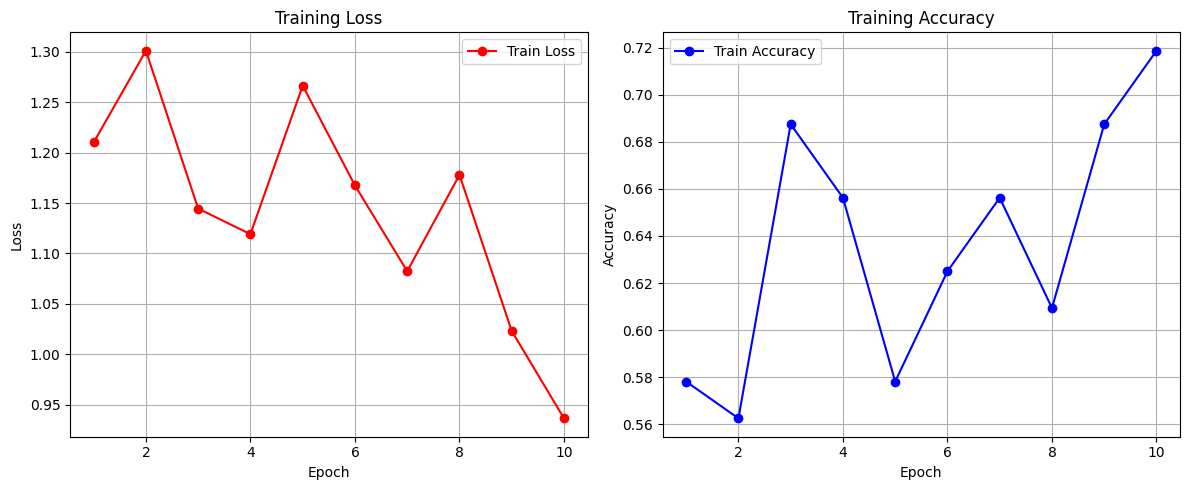
\includegraphics[width=0.9\textwidth]{assets/cassava/custom_acc_loss.png}
    \caption{Accuracy and Loss Curves of Custom CNN Model without Early Stopping}
\end{figure}

\begin{figure}[H]
    \centering
    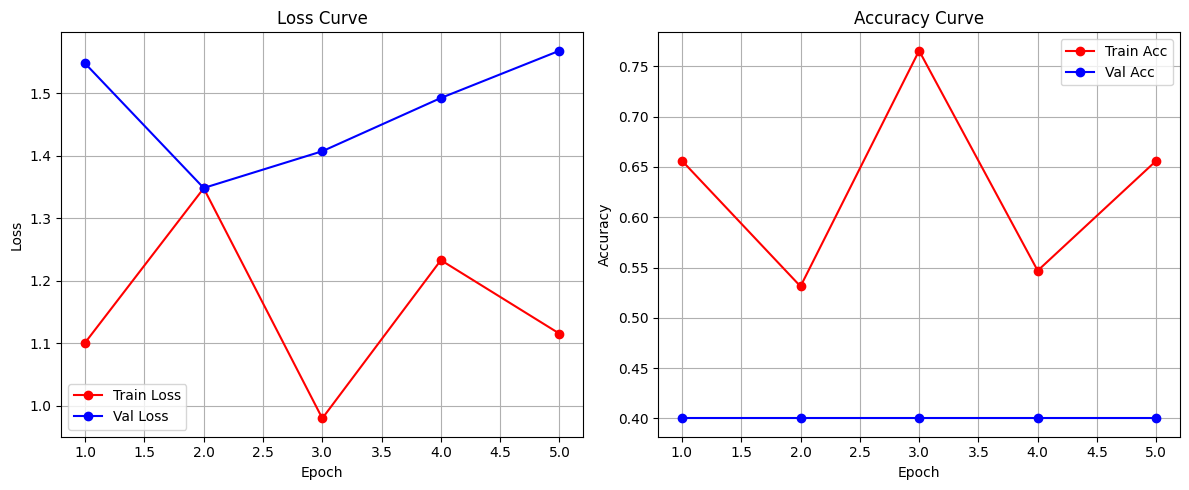
\includegraphics[width=0.9\textwidth]{assets/cassava/early_custom_loss_accu.png}
    \caption{Accuracy and Loss Curves of Custom CNN Model with Early Stopping}
\end{figure}

\begin{verbatim}
# Training results
Epoch 1/10 | Train Loss: 1.1012 | Train Acc: 0.6562 | Val Loss: 1.5481 | Val Acc: 0.4000
Validation loss improved, saving model...
Epoch 2/10 | Train Loss: 1.3483 | Train Acc: 0.5312 | Val Loss: 1.3487 | Val Acc: 0.4000
Validation loss improved, saving model...
Epoch 3/10 | Train Loss: 0.9801 | Train Acc: 0.7656 | Val Loss: 1.4076 | Val Acc: 0.4000
No improvement in validation loss for 1 epoch(s)
Epoch 4/10 | Train Loss: 1.2332 | Train Acc: 0.5469 | Val Loss: 1.4928 | Val Acc: 0.4000
No improvement in validation loss for 2 epoch(s)
Epoch 5/10 | Train Loss: 1.1156 | Train Acc: 0.6562 | Val Loss: 1.5685 | Val Acc: 0.4000
No improvement in validation loss for 3 epoch(s)
Early stopping triggered!
\end{verbatim}


\clearpage % Ensure clean page break before next section
\subsection*{Pre-trained ResNet50 Model}
\begin{lstlisting}
# Preprocess Data
Load label map (5 classes)
Apply train transforms: resize 224x224, random rotation, flip, affine, normalize
Apply val/test transforms: resize 224x224, normalize
Load dataset, split: 1000 train, 10 val, 200 test
Create data loaders: batch 32 (train), 10 (val), 32 (test)

# Early Stopping
Monitor val loss, patience 10, restore best weights

# Model
Load pre-trained ResNet50, exclude top
Freeze conv layers
Add: GlobalAvgPool2D, Dense(128, ReLU), Dropout(0.5), Dense(5, softmax)

# Train
Compile: Adam, crossentropy, accuracy
Train 50 epochs, batch 32
For each epoch:
  Train: forward, loss, backward, update weights
  Validate: compute loss, accuracy
  Early stop: save best weights if val loss improves, stop after 10 no-improvement
Store history: train/val loss, accuracy
Plot learning curves
\end{lstlisting}


\subsection*{Pre-trained ResNet50 Performance}
\begin{figure}[H]
    \centering
    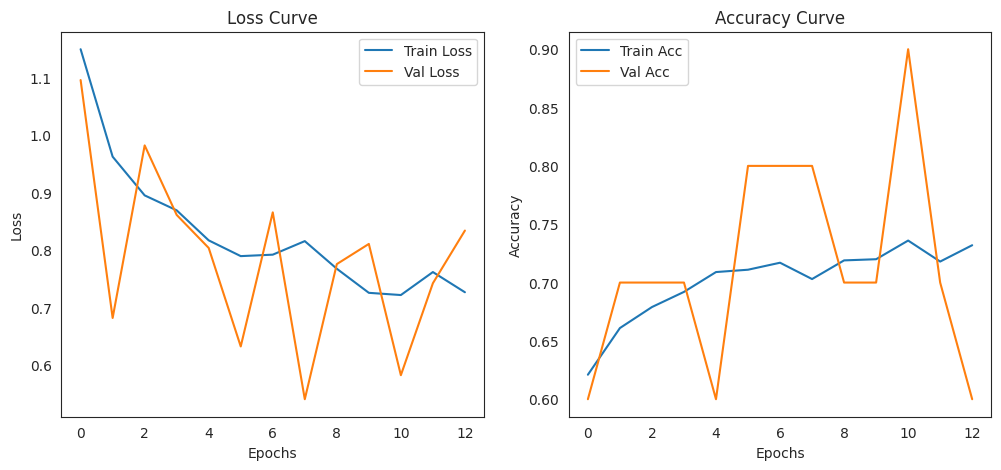
\includegraphics[width=1.0\textwidth]{assets/cassava/resnet_50.png}
    \caption{Accuracy and Loss of Pre-trained ResNet50 Model (Adam Optimizer)}
\end{figure}
\clearpage
\begin{lstlisting}
# Detailed Training Summary: ResNet50 Image Classification
Dataset: 16,898 images, 5 classes
Split: 1000 train, 10 val, 200 test
Device: CUDA
Setup: Pre-trained ResNet50, frozen conv layers, custom classifier
Training: 13/20 epochs (early stopping, patience 5)
- Batch Size: 32 (train, 32 batches), 10 (val, 1 batch)
- Optimizer: Adam (lr=0.001), Loss: Crossentropy, Metric: Accuracy

# Training Metrics
- Train Loss: 1.1499 (epoch 1) -> 0.9627 (epoch 2) -> 0.7896 (epoch 6) -> 0.7266 (epoch 13)
- Train Acc: 62.1% (epoch 1) -> 66.1% (epoch 2) -> 71.7% (epoch 7) -> 73.2% (epoch 13)
- Batch Loss Range: epoch 1: 0.7360-1.6883, stabilizes later
- Batch Acc Range: epoch 1: 21.88%-62.1%, stabilizes ~70% by epoch 13

# Validation Metrics
- Val Loss: 1.0962 (epoch 1) -> 0.6819 (epoch 2) -> 0.6322 (epoch 6) -> 0.5403 (epoch 8, best) -> 0.8341 (epoch 13)
- Val Acc: 60% (epoch 1) -> 70% (epoch 2) -> 80% (epoch 6) -> 90% (epoch 11) -> 60% (epoch 13)
- Best Model: Saved at epoch 8 (val loss 0.5403), restored after early stopping

# Early Stopping
- Triggered at epoch 13 (no val loss improvement after epoch 8)
- Patience: 5 epochs (pseudocode suggests 10)
- Val Loss Progression: 0.5403 (epoch 8) -> 0.7757 (9) -> 0.8108 (10) -> 0.5822 (11) -> 0.7424 (12) -> 0.8341 (13)

# Observations
- Steady train loss reduction (~37%) and acc improvement (~18%)
- Val metrics unstable due to small val set (10 samples)
- Possible premature stopping due to strict patience (5 epochs)
- Deprecated 'pretrained' parameter used
\end{lstlisting}
\clearpage
\section*{Optimizers}
\begin{itemize}
    \item \textbf{Adam}: Used for all models, offering fast convergence via adaptive learning rates.
    \item \textbf{SGD}: Used for the diabetes model, providing stable but slower convergence.
\end{itemize}

\section*{Findings}
\begin{itemize}
    \item \textbf{Diabetes Dataset}:
    \begin{itemize}
        \item The regularized model with dropout and batch normalization improved generalization.
        \item SGD provided stable performance, potentially outperforming Adam in F1-score.
        \item Early stopping was critical to prevent overfitting.
    \end{itemize}
    \item \textbf{Cassava Dataset}:
    \begin{itemize}
        \item Data augmentation (rotation, flip, zoom) enhanced model robustness, as evidenced by augmented images.
        \item The pre-trained ResNet50 model outperformed the custom CNN due to its pre-trained features.
        \item Early stopping and dropout effectively controlled overfitting.
    \end{itemize}
    \item \textbf{Decision}: Use the regularized model with SGD for diabetes prediction and the pre-trained ResNet50 model with data augmentation for cassava disease classification.
\end{itemize}

\clearpage

\end{document}
